\chapter{Introduction} \label{chap:intro}
The goal of this thesis is the implementation of a parallel implementation of a pointer analysis. As well as researching to what extent such an implementation presents advantages or disadvantages over other analyses that are not strictly parallel in nature.
\begin{center}
    \textbf{A digital version of this thesis together with the full source code of the developed software is available online at TODO\\
        \href{https://git.informatik.uni-kiel.de/stu210239/masterarbeit}{https://git.informatik.uni-kiel.de/stu210239/masterarbeit}.}
\end{center}
\section{Structure of this Thesis}
This thesis is divided into three chapters.
The first chapter \autoref{chap:intro} lays the groundwork for the implementation and goes into detail what ideas were pursued in order to develop the implementation. All related current work and its influences on this thesis are discussed here, as well as the motivation for the implementation itself. Furthermore, the fundamentals of pointer analysis are explained here with code samples and an end to end analysis workflow that aims to illustrate the connection between actual code and its representation in a pointer analysis.

In the second chapter \autoref{chap:main} the software, namely PTAGPU, that was developed as part of this thesis, is described in detail. Design decisions, integrations with other software libraries and correctness are elaborated here.
The experimental benchmark results and how they were generated are also presented here.

The last chapter \autoref{chap:conclusion} covers possible future work that could further improve the implementation and explore more ideas concerning parallel pointer analyses.
This chapter also discusses the experimental results from \autoref{chap:main}.

\section{Motivation}
This thesis aims to explore the possibilities of parallelizing the Andersen style inclusion-based whole program pointer analysis. Specifically the goal is to improve static pointer analysis performance by using massively parallel GPGPUs.
With the general trend of more complex software systems in software development, developers also require static analysis tools that are able to perform scalable analyses on entire codebases.
Unfortunately general pointer analysis is an undecidable computational problem \cite{landi1992undecidability}, which prevents fully precise pointer analyses from being a possibility.
For this reason all pointer analyses are approximate, and a balance must be found between performance and precision when analyzing code.
Historically most pointer analysis solutions have been implemented as single threaded applications, because pointer analyses are challenging to parallelise \cite{su2015efficient}. By using GPGPUs the proposed library from this thesis aims to improve performance when analyzing entire programs by distributing the work across the many streaming processors modern GPGPUs possess. The performance improvement of the proposed implementation also do not decrease the analysis precision.
\subsection{Static Analysis in Software Development}
Currently, most compilers employ almost entirely intraprocedural pointer analyses to allow for a fast and scalable static analysis during compilation. Only recently limited support for interprocedural analyses was introduced in the GCC compiler\footnote{\url{https://gcc.gnu.org/onlinedocs/gcc-12.2.0/gcc/Static-Analyzer-Options.html}}.
With greater complexity in modern software projects, these ad hoc intraprocedural analyses during compilation are not sufficient for finding most bugs because they suffer from low accuracy and missing semantic information \cite{gu2020towards}.
Especially if a software project is composed of many components, interprocedural analysis is required for finding bugs that arise from interactions between individual components.
One such project is the Linux kernel, which consists of a number of subcomponents that handle various parts of the kernel, such as drivers, cryptography and file systems.
While utilizing static analysis tools on the Linux kernel is nothing new, precise interprocedural analysis still is a challenging problem for almost 30 million lines of code in the Linux kernel.
For this reason this thesis explores options for improving scalability and performance of pointer analysis methods.

\section{Pointer Analysis}\label{sec:pta}
In general a pointer analysis tries to find the values of pointers in a program at runtime, without having to execute the program.
So naturally this problem is undecidable \cite{landi1992undecidability} following a reduction from the halting problem.
As a result, performing a pointer analysis becomes a delicate balancing act between precision and performance.
Commonly analyses produce over-approximations of the targets each pointer can point towards at runtime while other parts of an analysis might omit or under-approximate certain parts for the sake of performance and scalability.
As a result, these analyses are strictly speaking unsound or soundy as put forward by \cite{livshits2015defense}:

\begin{quote}
    We introduce the term soundy for
    such analyses. The concept of soundiness
    attempts to capture the balance,
    prevalent in practice, of over-approximated
    handling of most language features, yet deliberately
    under-approximated handling of a feature subset well
    recognized by experts. Soundiness is in
    fact what is meant in many papers that
    claim to describe a sound analysis. A
    soundy analysis aims to be as sound as
    possible without excessively compromising
    precision and/or scalability.
\end{quote}

Pointer analyses build the foundation for a variety of other static analyses, since call-graph generation is directly dependent on pointer analysis in order to resolve indirect or dynamic calls statically.

One common pointer analysis is the inclusion-based Andersen analysis \cite{andersen1994program}. The details of this type of analysis will be discussed later on, as it is the underlying basis for the proposed algorithm in \autoref{chap:main}. The Andersen algorithm sacrifices precision in favor of performance and achieves an upper bound of $O(n^3)$ where n represents the number of pointer variables relevant to the analysis. This is known as the cubic bottleneck of general Andersen analysis \cite{mathiasen2021fine}.
This showcases the trade-off that all non-theoretical pointer analyses have to make in order to be applicable to real programs and avoid undecidability. Furthermore, Andersen's analysis is a P-complete problem and is therefore not trivially parallelizable \cite{mathiasen2021fine}.

As a general abstraction, pointer analyses can be seen as complex graph problems where programs are interpreted as graphs with nodes representing variables and edges representing relations between nodes, such as memory allocations and assignments between variables.
This allows us to make use of a large body of previous research concerning graph problems and transform the general analysis into a better defined mathematical problem.

Another analysis closely related to pointer analysis is alias analysis, where two pointers are said to alias if their points-to sets have an intersection. An alias analysis produces a set of relations over all nodes in the analysis graph where nodes can either \textbf{NotAlias}, \textbf{MayAlias} or \textbf{MustAlias}.
For two given nodes, $a$, $b$ and their points-to sets $pts(a)$ and $pts(b)$ the following constraints describe the relations.
\begin{align}
    a\ \textbf{NotAlias}\ b \iff \forall ptd \in pts(a) \colon ptd \notin pts(b)\label{eq:alias1} \\
    a\ \textbf{MayAlias}\ b \iff \exists ptd \in pts(a) \colon ptd \in pts(b)\label{eq:alias2}    \\
    a\ \textbf{MustAlias}\ b \iff \forall ptd \in pts(a) \colon ptd \in pts(b)
\end{align}
Both pointer analysis, alias analysis, and points-to analysis are all terms commonly used interchangeably in literature \cite{hind2001pointer}. From now on pointer analysis will be used in this thesis to refer to this type of static analysis from which an alias relation can be derived based on the pointer information.

A motivating example for pointer analyses is the detection of memory leaks in programs.
This occurs when a memory location is allocated on the heap, for example with a call to \verb|malloc| in glibc, and is not freed at a later stage in the program.
It is in the interest of the developer to find such faults as to not exhaust the computer's memory during execution by repeatedly allocating memory in the heap without freeing previous allocations.
Finding such logical errors can be accomplished via a related static analysis called data-flow analysis, where each possible value at different stages of the program is calculated. Here pointer information is vital, as pointers can represent lateral movement of data through the control flow of a program, independent of direct assignments and read operations. Ultimately almost all static analyses require some kind of information about pointers to fully determine the state of a program.
Aside from error detection such as memory leaks, optimizations are another aspect of compiler systems, where pointer information is important to achieve better results, see \autoref{lst:dataflow}.
More often than not the pointer information alone does not provide an immediate value to the compiler or analysis tool, instead other procedures build on top of this information to derive valuable information about a program.

\begin{listing}
    \begin{minted}{c}
    #include <stdlib.h>
    void *iter;
    iter = value;

    /* depending on the data at value's memory location 
    the loop might not be necessary */
    
    while(*iter)
    {
        complex_computation(iter);
    }
    \end{minted}
    \caption{Optimizations in a c program}
    \label{lst:dataflow}
\end{listing}

\subsection{Notions of Sensitivity in Pointer Analysis}
As previously established, a complete pointer analysis is undecidable.
For this reason there are various notions of sensitivity when talking about pointer analysis.
These notions represent a compromise between precision, scalability and complexity of the analysis.
Following, some of the more common sensitivity notions will be illustrated to differentiate the more complex analyses from the less complex analyses and explain the impact of these sensitivities on actual performance when analyzing a program.

\subsubsection{Field-sensitivity}

\begin{listing}
    \begin{minted}{c}
    int a;
    char b;
    struct Person {
        char *name;
        int *age;
    } p1, p2;
    p1.age = &a;
    p1.name = &b;
        \end{minted}
    \caption{Field-sensitivity by example}
    \label{lst:field}
\end{listing}

Field-sensitivity describes how the pointer analysis algorithm handles structures in the program.
Most programming languages that expose memory management to a developer, such as c, c++ and Rust, offer some form of structures to represent an object that internally holds multiple values where these values might be pointers, that reference memory locations.
If an analysis is field-sensitive, each field of each struct is represented in the analysis as an independent node that can point to unique memory locations, as long as the field can be statically determined during the analysis, see \autoref{lst:field}.
If the field of a struct can not be statically determined, for example because of an arithmetic operation that produces multiple possible results for the offset during runtime, it is common for field-sensitive pointer analyses to fall back to a field-insensitive mode for the specific struct, wherein all fields of the struct are merged into a single abstract object.
For the given example, \verb|p1.age| and \verb|p1.name| can point to different memory locations.
Alternatively a field-insensitive analysis does not differentiate between any fields of a given struct at any point of the analysis.
Therefore, only two nodes are created to represent the struct, $p1.*$ and $p2.*$.
Another common alternative is field-base-sensitivity, where instead of omitting the individual fields of each struct, the fields of every struct are merged into a single instance of that struct.
As a result the Person structs, p1 and p2, would be represented as a single object with fields name and age, such that \verb|p1.age == p2.age| are represented by the same node in the analysis.

\subsubsection{Array-sensitivity}
Array-sensitivity is conceptually similar to field-sensitivity but often has different effects on the runtime of the analysis.
For a given array $int arr[100]$ an array-sensitivie analysis would model each entry of the array, \newline e.g. arr[0], arr[1], \dots, with a unique node, whereas an insensitive analysis would model the array as a single node.
Generally speaking arrays are often homogeneous data structures that can hold a vast amount of data, compared to structs which are often more compact as they model attributes instead of raw data.
Therefore, array-sensitivity if often omitted from whole program analyses, while field-sensitivity is common among pointer analyses.

\subsubsection{Scope of the analysis}
When designing a pointer analysis one has to make a decision about how to handle external code that the program depends on.
Often times transitive dependencies of a program can dwarf the original code by several magnitudes in size \cite{toman2017taming}.
Even a basic Hello World program in Java transitively depends on 3000 classes \cite{kulkarni2016accelerating} from the Java standard library.
For this reason most analyses either ignore external library code during analysis, or stub the most relevant library calls during analysis, such as \verb|malloc| or \verb|free|.
This trade-off is well worth it, as most interesting properties in pointer analysis do not originate in external libraries, but the actual program code that is written by the developer.
This does however not solve the problem of standard library code mutating the program state either via callbacks or mutation of values behind pointer arguments. Here, simply ignoring the external code during analysis would greatly decrease the accuracy of the analysis.
For this reason, a lot of research is being done to develop methods that alleviate some of the problems that arise from analyzing external dependencies of a given program. Caching incremental results during analysis seems to be one of the most promising methods thus far \cite{mcpeak2013scalable}, where instead of solving the pointer analysis problem from the top-down, the analysis begins at the bottom and builds summaries for functions incrementally until a result over the entire program is achieved. Hybrid approaches combining top-down and bottom-up analysis represent state-of-the-art analysis methods in use by production static analysis tools, such as Coverity \cite{mcpeak2013scalable}.

\subsubsection{Interprocedural analysis}
Another aspect that greatly influences the precision of analyses is whether they are interprocedural or intraprocedural.
An intraprocedural analysis only analyzes each function in an isolated context and disregards any influences on other functions or global state.
Interestingly most compilers rely mostly on intraprocedural analysis for bug detection as it can be performed in parallel for each function independently and is in general much faster than interprocedural analysis.
The following example \autoref{lst:intraprocedural} illustrates the shortcomings of only performing intraprocedural analysis. Essentially parameter passing especially of pointers is not taken into account properly for the calculation of points-to sets.
An interprocedural analysis overcomes these limitations by connecting parameters of functions and the arguments at the respective call-sites as well as the resulting return values in the graph structure that is used to solve the pointer analysis.
Fundamentally an interprocedural analysis is related to another notion of sensitivity, context sensitivity, since every context-sensitive analysis has to be interprocedural in order to capture the context of each function call \cite{lin2015alias}.

\begin{listing}
    \begin{minted}{c}
        int *manupulatePointer(int *ptr);
        int main() {
            int *a, *b;
            b = manupulatePointer(a);
            /* intraprocedural analysis is unable 
            to determine the state of a or b */
        }
    \end{minted}
    \caption{Limitations of intraprocedural analysis}
    \label{lst:intraprocedural}
\end{listing}

\subsubsection{Flow-sensitivity}
When one performs a flow-sensitive pointer analysis, this means that the analysis takes into account the control flow of the program when calculating point-to information.
As can be seen in \autoref{lst:flowsens}, a flow-sensitive analysis is in general more precise than a flow-insensitive analysis. Meanwhile, running a flow-sensitive analysis is also exponentially more expensive to compute as every step in a programs control flow carries its own state concerning points-to relations - especially when the control flow is complicated by complex conditional statements or recursive execution.
Although this problem can be slightly alleviated, by only considering program statements that manipulate pointers.
Empirical studies have shown that for context-insensitive analyses, adding flow-sensitivity to the points-to calculation does not offer a significant precision improvement over flow-insensitive analyses \cite{hind2001pointer}. This makes using a flow-sensitive analysis without context-sensitivity unattractive as an initial analysis run. One should rather combine context- and flow-sensitivity in subsequent analysis runs to refine the initial points-to results in certain regions of code that profit from a further refinement.
Using a flow-sensitive pointer analysis also generates must-alias relations, compared to the comparatively imprecise may-alias relations from a flow-insensitive pointer analysis.
Generating definitive information that two variables will unconditionally alias during runtime is very valuable when considering refactoring optimizations by a compiler.
While a sound may-alias analysis requires that no possible alias relations are missed, a sound must-alias analysis requires analogously that no spurious alias relations are reported. Both are respectively over- and under-approximations of the true points-to results.

\begin{listing}
    \begin{minted}{c}
        int *manupulatePointer(int *ptr);
        int main() {
            int a, b, *x; // x -> {}
            if (something())
                x = &a; // x -> {a}
            else
                x = &b; // x -> {a,b} ?
            manupulatePointer(x);
            /* a flow insensitive analysis computes 
            a points-to set {a,b} for x while in actuality 
            x = &b and x = &a are mutually exclusive statements
            during execution */
        }
    \end{minted}
    \caption{Flow-sensitivity by example}
    \label{lst:flowsens}
\end{listing}

\subsubsection{Context-sensitivity}
As previously alluded to, context-sensitivity is directly related to interprocedural analyses, since it governs how call sites and called functions are interpreted during the analysis.
More specifically a context-sensitive analysis tries to qualify variables both on the heap and stack with contextual information such that different contexts can be established, where for example points-to information for a variable differs, thus improving the precision of the analysis.
To achieve this context-sensitivity can be modeled by using call-sites and objects to differentiate qualify the context for variables \cite{smaragdakis2015pointer}. Depending on the programming language at hand, these methods can yield different precision. It has been established that object-oriented languages like Java greatly benefit from object-sensitivity over call-site-sensitivity, while more procedural languages like C benefit from call-site-sensitivity.
While a context-sensitive analysis would in theory provide more precision and therefore decrease the average size of points-to sets, in practice most context-sensitive pointer analyses, when applied to sizeable codebases, quickly grow out of control as the analysis explodes in terms of running time and space requirements \cite{smaragdakis2014introspective}. In contrast, context-insensitive analyses anecdotally scale better than context-sensitive analyses.

\begin{listing}
    \begin{minted}{c}
        int *manupulatePointer(int *ptr);
        int main() {
            int a, b, *x;
            x = &a;
            manupulatePointer(x);
            x = &b;
            manupulatePointer(x);
            /* a context-sensitive analysis evaluates both
            calls to manupulatePointer as unique function calls
            since the context differs between both calls */
        }
    \end{minted}
    \caption{Context-sensitivity by example}
    \label{lst:contextsens}
\end{listing}

\subsection{Andersen's Analysis}\label{sec:ander}
Andersen's analysis is an inclusion-based interprocedural pointer analysis algorithm first proposed by \cite{andersen1994program} in 1994. It is a field-sensitive, context-insensitive and flow-insensitive analysis. 
The algorithm was one of the first constraint based algorithms introduced for pointer analysis. Since it is lacking constext- and flow-sensitivity, it is often used as a base algorithm which produced broad over estimations of the points-to data and is later refined by more precise algorithms which improve the quality of the data and remove false positives from the points-to information generated by Andersen's algorithm.
The underlying idea is that the Algorithm operates on a given program by converting statements from the program into mathematical constraints contained in a constraint graph.
These constraints can be classified into a few types which can be seen in \autoref{tab:ander}.
It is worth noting that in literature the field-sensitivity aspect is often omitted from the definition of the Andersen analysis, although it was included in the original specification.
As mentioned in \autoref{chap:intro} the complexity of Andersen's analysis grows exponentially in regard to the number of pointer variables in a program. The reason for this exponential growth, among other aspects, is the field-sensitivity. Depending on the structure of the code under analysis, field-sensitivity might play the most influential part in the analysis' complexity. This will be further expanded upon in \autoref{chap:main}. Ultimately this is the reason for specifically including field-sensitivity when discussing Andersen's analysis in this thesis.
During execution an Andersen style pointer analysis repeatedly applies the constraints until a point is reached where no more changes are applied to the constraint graph at which point the execution concludes and the points-to sets for each variable are returned.
\begin{table}
    \begin{center}
        \begin{tabular}{l|l|l|l}
            \hline                                                                                                                          \\
            \textbf{Statement} & \textbf{Name} & \textbf{Description}                    & \textbf{Constraint}                              \\
            \hline                                                                                                                          \\
            $x = \&a$          & alloca        & \makecell[cl]{The address of a is                                                          \\assigned to x.}  & $\{a\} \subseteq pts(x)$                    \\
            $x = y$            & copy          & \makecell[cl]{Variable y is assigned                                                       \\to x.}            & $pts(y) \subseteq pts(x)$                        \\
            $x = *y$           & load          & \makecell[cl]{Load value of y and                                                          \\assign to x.}       & $\forall p \in pts(y) \colon pts(p) \subseteq pts(x)$ \\
            $*x = y$           & store         & \makecell[cl]{Store y into value of x.} & $\forall p \in pts(x) \colon pts(y) \subseteq pts(p)$ \\
            $x = y.f$          & field         & \makecell[cl]{Field f of variable y is                                                     \\assigned to x.} & $pts(y.f) \subseteq pts(x)$                      \\
        \end{tabular}
    \end{center}
    \caption{Constraints of an inclusion-based pointer analysis.}
    \label{tab:ander}
\end{table}

\subsection{Steensgard's Analysis}
Steensgard's analysis was introduced in 1996 by \cite{steensgaard1996points}. It was inspired by Andersen's analysis and as such is also an interprocedural pointer analysis.
The key proposition of Steensgard's work was to improve the runtime of Andersen's algorithm by using equalities instead of subsets for the constraints that are used as inputs for the algorithm, an overview for the constraints can be seen in \autoref{tab:steens} - the rules are nearly identical to the constraints for the Andersen algorithm.
The change from subsets to equalities leads to an almost linear algorithm by utilizing union/find data structures for efficient computation of a fixpoint solution for a given set of pointers.
The trade-off for this faster algorithm is precision, since Steensgard's algorithm quickly loses precision compared to Andersen's algorithm by losing the small differences between points-to sets of individual variables by equating them. An example for this precision loss can be seen in \autoref{lst:steensvander}.

\begin{listing}
    \begin{minted}{c}
        int main() {
            int a, b, *x, *y;
            x = &a; // pts(x) = {a}
            y = &b; // pts(y) = {b}
            y = x; // pts(y) = pts(x) = {a,b}
            /* by equating the points-to sets of x and y
            the fact that x never points to b is lost
            this leads to an obvious loss of precision */
        }
    \end{minted}
    \caption{Steensgard easily looses precision.}
    \label{lst:steensvander}
\end{listing}

\begin{table}
    \begin{center}
        \begin{tabular}{l|l|l|l}
            \hline                                                                                                                  \\
            \textbf{Statement} & \textbf{Name} & \textbf{Description}                    & \textbf{Constraint}                      \\
            \hline                                                                                                                  \\
            $x = \&a$          & alloca        & \makecell[cl]{The address of a is                                                  \\assigned to x.}  & $pts(x) = \{a\} \cup pts(x)$                    \\
            $x = y$            & copy          & \makecell[cl]{Variable y is assigned                                               \\to x.}            & $pts(y) = pts(x)$                        \\
            $x = *y$           & load          & \makecell[cl]{Load value of y and                                                  \\assign to x.}       & $\forall p \in pts(y) \colon pts(p) = pts(x)$ \\
            $*x = y$           & store         & \makecell[cl]{Store y into value of x.} & $\forall p \in pts(x) \colon pts(y) = pts(p)$ \\
            $x = y.f$          & field         & \makecell[cl]{Field f of variable y is                                             \\assigned to x.} & $pts(y.f) = pts(x)$                      \\
        \end{tabular}
    \end{center}
    \caption{Constraints of an equality-based pointer analysis.}
    \label{tab:steens}
\end{table}

\subsection{Wave Propagation}
Since its first introduction in 1994, there have naturally been many incremental improvements to Andersen style pointer analysis.
Most current implementations are derived from \cite{waveprop}, specifically the Wave Propagation Method, which is a highly optimized version of Andersen's algorithm.
In Wave Propagation the procedure is separated into an insertion phase and a propagation phase. Furthermore, the constraint graph is topologically sorted and acyclic, which enables the algorithm to pass forward the computed points-to information in topological order, preventing redundant work since only set differences need to be propagated to the next nodes. The algorithm is intended to be more memory intensive in order to achieve better performance on large codebases \cite{waveprop}.
The general algorithm for wave propagation is listed in \autoref{alg:waveprop}.

\begin{algorithm}
    \caption[General Wave Propagation Algorithm]{General Wave Propagation Algorithm \\ \textbf{Input:} Constraint Graph $G=(V,E)$ \\ \textbf{Output:} Modified Constraint Graph $G=(V,E)$ and points-to information.}\label{alg:waveprop}
    \begin{algorithmic}
        \State Detect strongly connected components and find topological sorting for $G$. \\ Build topological node stack $T$.
        \Repeat
        \State changed = False
        \State worklist = $\emptyset$
        \While{$T \neq \emptyset $}
        \State node $\leftarrow$ pop from T
        \For{edge (node,target) $\in out_{copy/gep}(node)$}
        \State pts(target) $\leftarrow$ union pts(node) pts(target)
        \If{pts(target) changed}
        \State changed = False and add target to worklist
        \EndIf
        \EndFor
        \EndWhile
        \While{worklist $\neq \emptyset $}
        \State node $\leftarrow$ pop from worklist
        \For{edge (node,target) $\in out_{load}(node)$}
        \For{ptsDst $\in pts(node)$}
        \State add copy edge (ptsDst, target) to $G$.
        \If{edge added to $G$}
        \State changed = True
        \EndIf
        \EndFor
        \EndFor
        \For{edge (src,node) $\in in_{store}(node)$}
        \For{ptsDst $\in pts(node)$}
        \State add copy edge (src, ptsDst) to $G$.
        \If{edge added to $G$}
        \State changed = True
        \EndIf
        \EndFor
        \EndFor
        \EndWhile
        \If{Edge added to $G$}
        \State changed = True
        \EndIf
        \Until{changed = False}
    \end{algorithmic}
\end{algorithm}

\subsection{LLVM - Generating Data for the Analysis}
By now the fundamentals of pointer analysis have been introduced, which unilaterally can be modeled as a graph problem.
The missing part of the introduction is where the underlying data for such a pointer analysis algorithm comes from or how it is derived from a given program that has to be analyzed.
Initially pointer analyses were solely implemented in compilers to detect errors and find possible optimizations during compilation. As compilers already employ an internal representation for the programs to be compiled, the data generation was not problematic.
As the scope of pointer analyses expands from intraprocedural analysis part of a compiler towards standalone interprocedural whole program analyses it is clear, that a new representation for programs is needed, on which analyses can run - independent of compilations.

During initial review of literature for pointer analysis multiple methods for data generation were surveyed. Notably parsing was among the most common data extraction methods for programs. Another method was to extract an intermediate representation, called LLVM-IR, of the code during compilation of a program by means of using the low level virtual machine, LLVM. Using LLVM has some distinct advantages compared to parsing the source files of a program directly.
For one, LLVM provides multiple compiler front-ends for various compiled programming languages, including C/C++ and Objective-C through the Clang compiler, which allows one to compile multiple languages without having to adapt the parser, as can be seen in \autoref{fig:llvm}.
Especially when working with older non-strictly standardized versions of the C language, utilizing all available tricks of an established compiler proves to be more resourceful compared to reinventing the wheel with new parsing tools.
Secondly one can easily verify the correctness of the extracted data for a program by simply executing the compiled intermediate representation since no matter the programming language, as part of the LLVM toolchain the program always gets compiled into the intermediate representation before being assembled and linked. The LLVM project provides specific tools for executing programs in LLVM-IR format using a just-in-time compiler \footnote{https://releases.llvm.org/9.0.1/docs/CommandGuide/lli.html}. Beyond the binary intermediate representation, also called bitcode, there exists a human-readable format. Both binary and text versions can be converted between with the LLVM tools \verb|llvm-as| and \verb|llvm-dis|, see \autoref{lst:llvmir} for a basic hello world program in human-readable LLVM-IR.

\begin{figure}
    \centering
    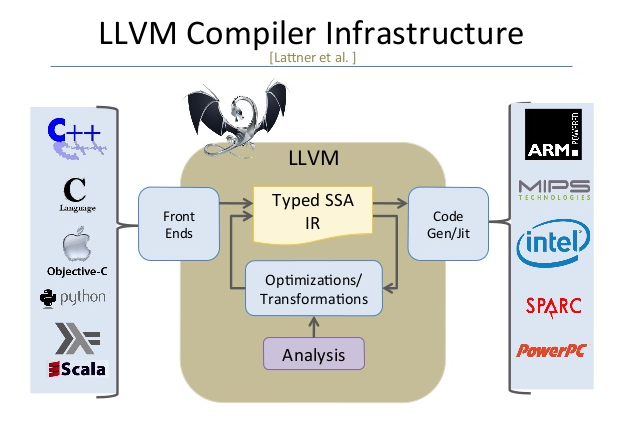
\includegraphics[width=.8\textwidth]{img/llvm.png}
    \caption{Illustration of the LLVM toolchain from Lattner et al.}
    \label{fig:llvm}
\end{figure}

\begin{listing}
    \begin{minted}{c}
#include <stdio.h>
int main()
{
    int i;
    i = 10;
    printf("Hello World! N = %d\n", i);
    return 0;
}
// gets compiled into...
    \end{minted}
    \begin{minted}{llvm}
@.str = private unnamed_addr constant 
    [21 x i8] c"Hello World! N = %d\0A\00", align 1
; Function Attrs: noinline nounwind optnone uwtable
define dso_local i32 @main() #0 {
  %1 = alloca i32, align 4
  %2 = alloca i32, align 4
  store i32 0, i32* %1, align 4
  store i32 10, i32* %2, align 4
  %3 = load i32, i32* %2, align 4
  %4 = call i32 (i8*, ...) @printf(i8* getelementptr inbounds 
        ([21 x i8], [21 x i8]* @.str, i64 0, i64 0), i32 %3)
  ret i32 0
}
declare dso_local i32 @printf(i8*, ...) #1
    \end{minted}
    \caption{A basic hello world program in human-readable LLVM-IR.}
    \label{lst:llvmir}
\end{listing}

\subsubsection{LLVM Instructions}
With the generated LLVM-IR we can now build a graph, by interpreting the individual LLVM instructions as constraints for a chosen pointer analysis.
The LLVM-IR uses static single assignment (SSA) form for variables meaning that each variable can only be assigned a single time in a specific control flow in the intermediate representation.
The use of SSA form is not directly relevant to Andersen style analyses but simplifies working with variables conceptually, since no variable can be reassigned at any point of the program.
At this point it is also important to differentiate between address-taken variables and top-level variables.
Top-level variables' values reside in registers and are conceptually ephemeral while address-taken variables are abstract memory objects which logically reside in memory. The specifics of memory locations and cpu registers are of cause hardware specific and depend on the target architecture that the LLVM backend assembles the intermediate representation into.
The connection between address-taken and top-level variables in the LLVM-IR is established by the \verb|alloca| instruction which maps a top-level variable to a memory location represented by an address-taken variable.
Following is an interpretation of the LLVM instructions for Andersen's pointer analysis.

\paragraph{Alloca Instruction}
The LLVM \verb|alloca| instruction is used to allocate memory on the stack.
\begin{minted}{llvm}
    ; allocate a pointer to a 32 bit integer on the stack 
    ; and save a reference at ptr
    %ptr = alloca i32*, align 8
\end{minted}
The analog of the \verb|alloca| instruction in a pointer analysis is the address-of operation $x = \&a$, since the top-level variable $ptr$ points to the abstract memory location holding the actual value.
This might come as a surprise, since the implementation of $x = \&a$ in C does not result in an \verb|alloca| instruction. This often leads to confusion when interpreting points-to results that are built using the LLVM-IR.

\paragraph{Load Instruction}
The LLVM \verb|load| instruction loads the value on a top-level variable into a new variable. Compared to the C programming language this is comparable to dereferencing a pointer variable.
\begin{minted}{llvm}
    %ptr = alloca i32*, align 8
    ; load the pointer to the 32 bit integer from ptr into %var
    %var = load i32*, i32** %ptr, align 8
\end{minted}
When interpreting LLVM load instructions for a pointer analysis, we can treat it as the complex load constraint that is already defined for Andersen's analysis in \autoref{tab:ander}.
Again just like the \verb|alloca| instruction we can not draw a direct comparison between the definition of the constraint $x = *y$ and the equivalent statement in the C language, since we are working with the LLVM-IR in SSA form.
The C equivalent would be the dereferencing of $*y$ alone. The assignment to x would require another store instruction.

\paragraph{Store Instruction}
The LLVM \verb|store| instruction stores a value into a variable. The variable might be a top-level or an abstract memory object represented by an address-taken variable.
\begin{minted}{llvm}
    %ptr = alloca i32*, align 8
    %var = load i32*, i32** %ptr, align 8
    ; store the literal value 10 into %var
    store i32 10, i32* %var, align 4
\end{minted}
The interpretation of the LLVM store instruction is similar to the load instruction. It can be interpreted as the complex store constraint defined as part of Andersen's analysis.

\paragraph{Getelementptr Instruction}
The LLVM \verb|getelementptr| or \verb|gep| instruction is used to get subelements from an aggregate data structure such as arrays or structs. When the gep instruction is invoked, it requires an index in order to perform the address calculation for the subelement. \verb|Getelementptr| does not access memory, it only finds the correct address.
\begin{minted}{c}
    int arr[10];
    arr[5] = 10;
\end{minted}
\begin{minted}{llvm}
    ; create an integer array
    %arr = alloca [10 x i32], align 16
    ; get the address for the 5th element
    %idx = getelementptr inbounds [10 x i32], [10 x i32]* %arr, 
        i64 0, i64 5
    store i32 10, i32* %idx, align 4
\end{minted}
Since we intend to run a static analysis, we need to consider the properties of the index value passed into the \verb|getelementptr| instruction.
Either the index is a constant value, and we can forward the \verb|gep| instruction together with the constant index into the static analysis,
or the index is a variable that is subject to change during execution, and we need to assume that every possible value can be realized during execution, i.e. every offset for an aggregate data structure might be referenced by such a \verb|gep| instruction and this information must be passed to the static analysis.
This behavior is handled by differentiating between two types of \verb|gep| constraints in the pointer analysis, normal- and variant-gep constraints. The former specifying a singular offset and the latter every possible offset for a given aggregate data type, since the value can not be statically determined.

\paragraph{Copy Instruction and equivalent Instructions}
Other than the complex store, load and the address-of constraints, the Andersen inclusion-based pointer analysis operates also on simple constraints, see line 2 in \autoref{tab:ander}. In terms of LLVM-IR instructions we are only interested in those instructions that manipulate pointers. In the LLVM-IR specification lots of instructions can result in values being moved, including pointers. Therefore, we group those instructions that can move values between symbols under the simple inclusion-based constraint.
The following instructions are interpreted as simple constraints:
\begin{itemize}
    \item \verb|Phi| instructions are part of the LLVM-IR to correctly resolve control flow. Depending on the conditional branch a new SSA variable is introduced that holds the resulting value from the branch.
          Since we are implementing a flow-insensitive pointer analysis we do not differentiate between control flows and simply interpret each phi instruction as a simple constraint connecting the conditional values to the resulting phi variable.
    \item \verb|Select| instructions serve a similar purpose as \verb|phi| instructions. Here a value is selected conditionally without creating branches. As such we interpret the \verb|select| instruction as a simple constraint.
    \item \verb|Call| instructions represent a function call. If the function call contains arguments the caller arguments and callee parameters need to be interpreted as a simple constraint. Beyond this, nothing is done to analyze the context of the function call, since we are performing a context-insensitive pointer analysis.
    \item Like the call instructions, \verb|ret| instructions are simply interpreted as simple constraints so the returned function value is included in the pointer analysis.
    \item \verb|ThreadFork| \verb|ThreadJoin| are not LLVM-IR instructions. But just like the \verb|call| and \verb|ret| instructions, these must be interpreted as function calls with simple constraints in the context of pointer analysis.
    \item Lastly there are various instructions that are straightforward to interpret as simple constraints, including \verb|bitcast|, \verb|ptrtoint|, \verb|constexpr|, \verb|extractvalue| and \verb|freeze| instructions. Furthermore, variable argument values and external library call parameters need to be handled like regular \verb|call| instructions.
\end{itemize}

Now with \verb|alloca|, \verb|load| and \verb|store| instructions introduced, we can analyze a basic example by applying Andersen constraints to perform a pointer analysis.
We are going to observe a simple c program, which will compile into the following LLVM-IR.
\begin{center}
    \begin{minipage}[t]{0.3\textwidth}
        \begin{minted}{c}
    int *p, x, *q;
    p = &x;
    q = p;
        \end{minted}
    \end{minipage}
    \begin{minipage}[t]{0.6\textwidth}
        \begin{minted}{llvm}
    %1 = alloca i32*, align 8
    %2 = alloca i32, align 4
    %3 = alloca i32*, align 8
    store i32* %2, i32** %1, align 8
    %4 = load i32*, i32** %1, align 8
    store i32* %4, i32** %3, align 8
        \end{minted}
    \end{minipage}
\end{center}
An example for applying the constraint rules according to the Andersen algorithm in \autoref{tab:ander} can be observed in \autoref{tab:applyander}.
The edge labels of the constraint graph are \verb|p|, \verb|s|, \verb|l|, \verb|c| corresponding to points-to (inverse alloca), store, load and copy constraints.
Furthermore, the copy edges are immediately converted into point-to edges in order to simplify the constraint graph in this example and reduce the number of steps.
\begin{table}
    \caption{Example for Applying Andersen Constraints}
    \centering
    \label{tab:applyander}
    \begin{tabular}{p{0.5\textwidth} c c}
        \toprule
        Code Snippet to analyze / comment                & Constraint Graph                   \\
        \midrule
        \begin{minipage}[t]{0.5\textwidth}
            \begin{minted}{llvm}
%1 = alloca i32*, align 8
%2 = alloca i32, align 4
%3 = alloca i32*, align 8
            \end{minted}
        \end{minipage}            & 
        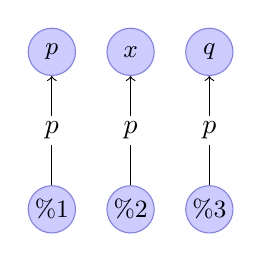
\begin{tikzpicture}[baseline=0]
            \tikzstyle{node}=[circle, draw=blue!50, fill=blue!20, inner sep=1pt, minimum size=6mm]
            \tikzstyle{linenode}=[pos=0.5,fill=white,inner sep=2pt,outer sep=2pt]
            \node[node] (A) at (0,-2) {\small$\%1$};
            \node[node] (B) at (1,-2) {\small$\%2$};
            \node[node] (C) at (2,-2) {\small$\%3$};
            \node[node] (Ap) at (0,0) {\small$p$};
            \node[node] (Bp) at (1,0) {\small$x$};
            \node[node] (Cp) at (2,0) {\small$q$};
            \path [->] (A) edge[] node[linenode] {$p$} (Ap);
            \path [->] (B) edge[] node[linenode] {$p$} (Bp);
            \path [->] (C) edge[] node[linenode] {$p$} (Cp);
        \end{tikzpicture} \\
        \midrule
        \begin{minipage}[t]{0.5\textwidth}
            \begin{minted}{llvm}
store i32* %2, i32** %1, align 8
            \end{minted}
        \end{minipage} & 
        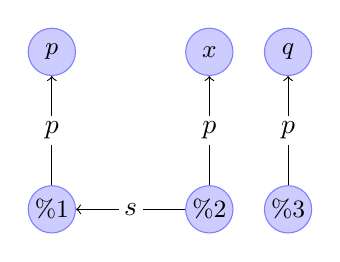
\begin{tikzpicture}[baseline=0]
            \tikzstyle{node}=[circle, draw=blue!50, fill=blue!20, inner sep=1pt, minimum size=6mm]
            \tikzstyle{linenode}=[pos=0.5,fill=white,inner sep=2pt,outer sep=2pt]
            \node[node] (A) at (0,-2) {\small$\%1$};
            \node[node] (B) at (2,-2) {\small$\%2$};
            \node[node] (C) at (3,-2) {\small$\%3$};
            \node[node] (Ap) at (0,0) {\small$p$};
            \node[node] (Bp) at (2,0) {\small$x$};
            \node[node] (Cp) at (3,0) {\small$q$};
            \path [->] (A) edge[] node[linenode] {$p$} (Ap);
            \path [->] (B) edge[] node[linenode] {$p$} (Bp);
            \path [->] (C) edge[] node[linenode] {$p$} (Cp);
            \path [->] (B) edge[] node[linenode] {$s$} (A);
        \end{tikzpicture} \\
        \midrule
        \begin{minipage}[t]{0.5\textwidth}
            \begin{minted}{llvm}
%4 = load i32*, i32** %1, align 8
store i32* %4, i32** %3, align 8
; create constraints from every 
; instruction
            \end{minted}
        \end{minipage} & 
        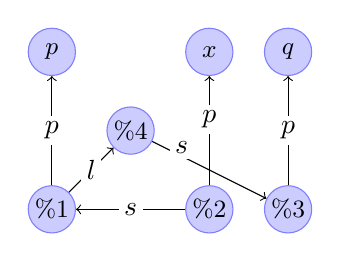
\begin{tikzpicture}[baseline=0]
            \tikzstyle{node}=[circle, draw=blue!50, fill=blue!20, inner sep=1pt, minimum size=6mm]
            \tikzstyle{linenode}=[pos=0.5,fill=white,inner sep=2pt,outer sep=2pt]
            \node[node] (A) at (0,-2) {\small$\%1$};
            \node[node] (B) at (2,-2) {\small$\%2$};
            \node[node] (C) at (3,-2) {\small$\%3$};
            \node[node] (Ap) at (0,0) {\small$p$};
            \node[node] (Bp) at (2,0) {\small$x$};
            \node[node] (Cp) at (3,0) {\small$q$};
            \node[node] (D) at (1,-1) {\small$\%4$};
            \path [->] (A) edge[] node[linenode] {$p$} (Ap);
            \path [->] (B) edge[] node[linenode, yshift=4pt] {$p$} (Bp);
            \path [->] (C) edge[] node[linenode] {$p$} (Cp);
            \path [->] (B) edge[] node[linenode] {$s$} (A);
            \path [->] (A) edge[] node[linenode] {$l$} (D);
            \path [->] (D) edge[] node[linenode, xshift=-10pt, yshift=8pt] {$s$} (C);
            % \draw[->, rounded corners=6mm] (E) -- ($(E.30) + (0.5,0.5)$) -- ($(Cp.30) + (0.4,0.4)$) node[linenode]{$s$} -- ($(C.30) + (0.5,0.5)$) -- (C);
        \end{tikzpicture} \\
        \midrule
        \begin{minipage}[t]{0.5\textwidth}
            \begin{minted}{llvm}
; apply first store 
; constraint rule(s)
            \end{minted}
        \end{minipage}               & 
        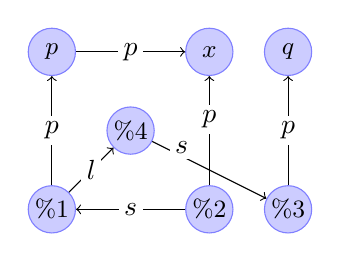
\begin{tikzpicture}[baseline=0]
            \tikzstyle{node}=[circle, draw=blue!50, fill=blue!20, inner sep=1pt, minimum size=6mm]
            \tikzstyle{linenode}=[pos=0.5,fill=white,inner sep=2pt,outer sep=2pt]
            \node[node] (A) at (0,-2) {\small$\%1$};
            \node[node] (B) at (2,-2) {\small$\%2$};
            \node[node] (C) at (3,-2) {\small$\%3$};
            \node[node] (Ap) at (0,0) {\small$p$};
            \node[node] (Bp) at (2,0) {\small$x$};
            \node[node] (Cp) at (3,0) {\small$q$};
            \node[node] (D) at (1,-1) {\small$\%4$};
            \path [->] (A) edge[] node[linenode] {$p$} (Ap);
            \path [->] (B) edge[] node[linenode, yshift=4pt] {$p$} (Bp);
            \path [->] (C) edge[] node[linenode] {$p$} (Cp);
            \path [->] (B) edge[] node[linenode] {$s$} (A);
            \path [->] (A) edge[] node[linenode] {$l$} (D);
            \path [->] (D) edge[] node[linenode, xshift=-10pt, yshift=8pt] {$s$} (C);
            % \draw[->, rounded corners=6mm] (E) -- ($(E.30) + (0.5,0.5)$) -- ($(Cp.30) + (0.4,0.4)$) node[linenode]{$s$} -- ($(C.30) + (0.5,0.5)$) -- (C);
            \path [->] (Ap) edge[] node[linenode] {$p$} (Bp);
        \end{tikzpicture} \\
        \midrule
        \begin{minipage}[t]{0.5\textwidth}
            \begin{minted}{llvm}
; apply last load and store 
; constraint rule(s)
; 
; finally p pts-to x
; and q also pts-to x
            \end{minted}
        \end{minipage}               & 
        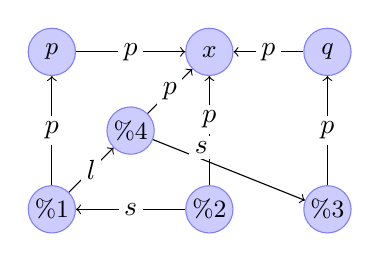
\begin{tikzpicture}[baseline=0]
            \tikzstyle{node}=[circle, draw=blue!50, fill=blue!20, inner sep=1pt, minimum size=6mm]
            \tikzstyle{linenode}=[pos=0.5,fill=white,inner sep=2pt,outer sep=2pt]
            \node[node] (A) at (0,-2) {\small$\%1$};
            \node[node] (B) at (2,-2) {\small$\%2$};
            \node[node] (C) at (3.5,-2) {\small$\%3$};
            \node[node] (Ap) at (0,0) {\small$p$};
            \node[node] (Bp) at (2,0) {\small$x$};
            \node[node] (Cp) at (3.5,0) {\small$q$};
            \node[node] (D) at (1,-1) {\small$\%4$};
            \path [->] (A) edge[] node[linenode] {$p$} (Ap);
            \path [->] (B) edge[] node[linenode, yshift=4pt] {$p$} (Bp);
            \path [->] (C) edge[] node[linenode] {$p$} (Cp);
            \path [->] (B) edge[] node[linenode] {$s$} (A);
            \path [->] (A) edge[] node[linenode] {$l$} (D);
            \path [->] (D) edge[] node[linenode, xshift=-10pt, yshift=8pt] {$s$} (C);
            % \draw[->, rounded corners=6mm] (E) -- ($(E.30) + (0.5,0.5)$) -- ($(Cp.30) + (0.4,0.4)$) node[linenode]{$s$} -- ($(C.30) + (0.5,0.5)$) -- (C);
            \path [->] (Ap) edge[] node[linenode] {$p$} (Bp);
            \path [->] (D) edge[] node[linenode] {$p$} (Bp);
            \path [->] (Cp) edge[] node[linenode] {$p$} (Bp);
        \end{tikzpicture} \\
        \bottomrule
    \end{tabular}
\end{table}

\section{Context-free Languages}
Looking at the problem definition for an Andersen style pointer analysis, most algorithms operate on graph data structures.
In this section we will look at an alternative interpretation of the pointer analysis problem where the problem can be solved by transforming it into a graph-reachability problem which can be solved by using context-free languages, i.e. CFL-reachability.
This approach was first introduced for static analysis purposes by \cite{reps1998program} and was found to be solvable in cubic time.

\subsection{Definition of Context-free Languages and Grammars}
A context-free language is a language that can be generated by a context-free grammar.
A context-free grammar is a 4-tuple $CFG=(V,\Sigma,R,S)$ that holds a finite set of nonterminal characters $V$, a finite set of terminal characters $\Sigma$, a finite relation (rewrite rules) over $V\times (V \cup \Sigma)^*$ and a start variable $S \in V$.

A prominent example for context-free languages is the balanced parenthesis language, which is defined by:
\begin{enumerate}
    \item $CFG_{bpar}=(V,\Sigma,R,S)$
    \item $V=\{S\}$
    \item $S=S$
    \item $\Sigma=\{(,)\}$
    \item $R=\{S\rightarrow\epsilon, S\rightarrow SS, S\rightarrow (S)\}$
\end{enumerate}
Given the grammar $CFG_{bpar}$ the language $\mathcal{L}_{bpar}(CFG_{bpar})$ is defined as all words that can be generated by the grammar or formally: $$\mathcal{L}_{bpar}(CFG_{bpar})= \{w\in \Sigma^* | S\Rightarrow_{CFG_{bpar}}^* w \}$$
Words that are part of $\mathcal{L}_{bpar}$ are for example \verb|(())| or \verb|(()())()|.
If we apply the concept of context-free languages to graphs, we can easily define a reachability relation based on context-free languages by interpreting edges as terminal characters and paths of edges, or concatenations of edge labels, as words - as long as the edge labels of a given graph are part of the alphabet for the context-free grammar.
Given the following graph $G$:
\begin{center}
    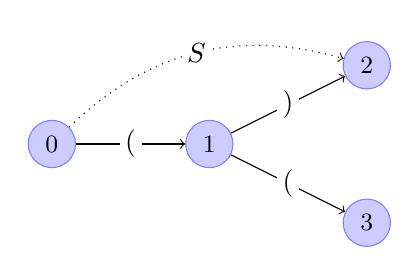
\begin{tikzpicture}[]
        \tikzstyle{node}=[circle, draw=blue!50, fill=blue!20, inner sep=1pt, minimum size=6mm]
        \tikzstyle{linenode}=[pos=0.5,fill=white,inner sep=2pt,outer sep=2pt]
        \node[node] (A) at (0,0) {\small$0$};
        \node[node] (B) at (2,0) {\small$1$};
        \node[node] (C) at (4,1) {\small$2$};
        \node[node] (D) at (4,-1) {\small$3$};
        \path [->] (A) edge[] node[linenode] {$($} (B);
        \path [->] (B) edge[] node[linenode] {$)$} (C);
        \path [->] (B) edge[] node[linenode] {$($} (D);
        \path [->] (A) edge[dotted, bend left] node[linenode] {$S$} (C);
    \end{tikzpicture}
\end{center}
The CFL-reachability defined by the grammar $CFG_{bpar}$ would find node 2 to be reachable by node 0, since the word "$()$" is part of $\mathcal{L}_{bpar}$.
This computed reachability can be saved in the graph, by inserting a new edge from node 0 to node 2 with the nonterminal label $S$, representing the balanced parenthesis property.
\subsection{Andersen Analysis via CFL-Reachability}\label{sec:ander-cfl}
With the knowledge about the Andersen constraints, a set of logical base facts along with terminal characters can be defined for each constraint as can be seen in \autoref{tab:cfl-ander}. Note that each terminal character $x$ also has an inverse representation $bar{x}$ which represents its inverse edge in the constraint graph.
With these base facts one can define horn-clause rules for a points-to relation \cite{reps1998program}. These horn-clauses can then be reinterpreted as a context-free grammar via the respective production rules that represent an instance of the Andersen pointer analysis problem, see \autoref{tab:cfl-ander2}.
$$R=\{P\rightarrow \bar{a}, C \rightarrow c, P\rightarrow aC, C\rightarrow al, C\rightarrow sP\}$$
$$CFG_{ander}=(\{P,C\}, \{a,c,l,s,\bar{a},\bar{c},\bar{l},\bar{s}\}, R, P)$$
With the context-free grammar the points-to information can then be computed by calculating the transitive closure of the points-to production rule $P$. In general a variable x points to a variable y iff a path $x \rightsquigarrow y$ exists such that the word created by the ordered edge labels of the path is in the language $\mathcal{L}(CFG_{ander})$ defined by the grammar.
In fact, most interprocedural static analyses can be implemented this way by using a context-free grammar.
The first time this approach was mentioned in the context of a pointer analysis was \cite{zheng2008demand} where context-free reachability was used to implement a demand-driven flow-insensitive alias analysis.
This proved to be a faster and more resource efficient approach compared to other demand-driven alias analyses at the time.
\begin{table}
    \begin{center}
        \begin{tabular}{l|l|l|l}
            \hline                                                                                 \\
            \textbf{Statement} & \textbf{Name} & \textbf{Base Fact}  & \textbf{Terminal Character} \\
            \hline                                                                                 \\
            $x = \&a$          & alloca        & alloca(a,x)         & a                           \\
            $x = y$            & copy          & simpleCopy(y,x)     & c                           \\
            $x = *y$           & load          & complexLoad(y,x)    & l                           \\
            $*x = y$           & store         & complexStore(y,x)   & s                           \\
            $x = y.f$          & field         & simpleField<N>(y,x) & f<N>                        \\
        \end{tabular}
    \end{center}
    \caption[Overview of CFG Terminals for Andersen Constraints]{Context-free Grammar Terminals and Base Facts for each Andersen Constraint.\\Field-sensitive base facts are implemented by a template e.g. one for each possible offset value N.}
    \label{tab:cfl-ander}
\end{table}

\begin{table}
    \begin{center}
        \begin{tabularx}{1\textwidth} {X|X|X}
            \hline                                                                   \\
            \textbf{Statement} & \textbf{Horn-clause rule}     & \textbf{Production} \\
            \hline                                                                   \\
            $x = \&a$          & \makecell[cl]{pointsTo(x,a):-                       \\\hspace{1em} alloca(a,x)} & $\{P\rightarrow \bar{a}\}$                          \\\hline
            $x = y$            & \makecell[cl]{pointsTo(x,a):-                       \\\hspace{1em} simpleCopy(y,x),\\\hspace{1em} pointsTo(y,a)} &$\{P\rightarrow \bar{c}P\}$    \\\hline
            $x = *y$           & \makecell[cl]{pointsTo(x,a):-                       \\\hspace{1em} complexLoad(y,x),\\\hspace{1em} pointsTo(y,z),\\\hspace{1em} pointsTo(z,a)}    & $\{P\rightarrow \bar{l}PP\}$                          \\\hline
            $*x = y$           & \makecell[cl]{pointsTo(a,b):-                       \\\hspace{1em} complexStore(y,x),\\\hspace{1em} pointsTo(x,a),\\\hspace{1em} pointsTo(y,b)}   & $\{P\rightarrow \bar{P}\bar{s}P\}$                          \\
        \end{tabularx}
    \end{center}
    \caption[Overview of CFG Productions for Andersen Constraints]{Context-free Grammar Productions and Horn-clauses for each Andersen Constraint.\\Field-sensitive rules are omitted for simplicity.}
    \label{tab:cfl-ander2}
\end{table}
\subsection{Context-free Path Queries via Matrix Multiplications}
While the transformation of the Andersen problem statement into a reachability relation on top of a context-free language is a helpful mathematical abstraction, it does nothing to improve performance, scalability or precision of the algorithm.
Subsequently, \cite{azimov2018context} proposed a matrix multiplication based approach that works with graph data and allows path queries by means of context-free grammars.
The general answer to a path query is a set of triples of the form $(P,a,b)$, such that there exists a path in the graph from node a to node b with a path labeling derived from the nonterminal P according to \cite{azimov2018context}.
The central idea for the algorithm is to solve these context-free path queries by calculating the transitive closure of matrices. These matrices are constructed by capturing the adjacency matrices of each individual terminal edge label from the graph. Given two of these boolean adjacency matrices, we can compute the transitive closure by repeatedly multiplying them until no more changes are applied.
To simplify these operations we can convert our context-free grammar that we derived from the Andersen constraints into Chomsky normal form.
After the conversion of a grammar $G=(V,\Sigma,R,S)$ into Chomsky normal form we are left with productions in the following form:
\begin{align}
     & P\rightarrow AB, & \textrm{ for } P,A,B \in V \label{eq:cnf1}               \\
     & P\rightarrow v,  & \textrm{ for } P \in V \land v\in \Sigma \label{eq:cnf2}
\end{align}
Following this, we iterate through all production rules in the form of \autoref{eq:cnf2} and populate the adjacency matrices, then we iterate through all production rules in the form of \autoref{eq:cnf1} and apply the matrix multiplications to find the transitive closures for each of these productions.
An elaborate proof for the correctness of this approach can be found in \cite{azimov2018context}.
Note that the cited paper uses a singular matrix containing sets for all edge relations between nodes instead of multiple boolean matrices for each edge type.
This does not have any effect on the correctness of the algorithm and simply improves the performance, since boolean matrices can be represented more efficiently than matrices of sets.
By rearranging the Andersen algorithm as repeated matrix multiplications, we indirectly profit from decades of research into efficient linear algebra algorithms.
In this case we utilize a subset of linear algebra algorithms, specifically sparse boolean linear algebra.
Whenever linear algebra is involved, it is often a good idea to use accelerators such as GPGPUs to speed up the calculations.

Next we will consider a basic pointer analysis example to illustrate the context-free path query approach that uses matrices for the calculation.
The input constraint graph that we will use as an input for the Andersen style analysis is derived from the following c code:

\begin{center}
    \begin{minipage}[t]{0.3\textwidth}
        \begin{minted}{c}
int main()
{
    int *p, x, *q;
    p = &x;
    q = p;
}
        \end{minted}
    \end{minipage}
    \begin{minipage}[t]{0.6\textwidth}
        \begin{minted}{llvm}
define dso_local i32 @main() #0 {
    %1 = alloca i32*, align 8 ; p
    %2 = alloca i32, align 4 ; x
    %3 = alloca i32*, align 8 ; q
    store i32* %2, i32** %1, align 8
    %4 = load i32*, i32** %1, align 8
    store i32* %4, i32** %3, align 8
    ret i32 0
}
        \end{minted}
    \end{minipage}
\end{center}
Which results in the following graph.
\begin{center}
    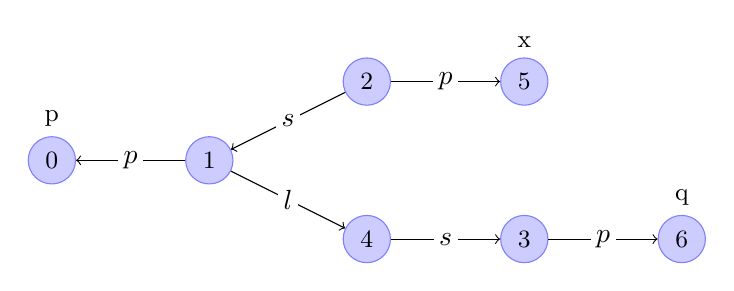
\begin{tikzpicture}[]
        \tikzstyle{node}=[circle, draw=blue!50, fill=blue!20, inner sep=1pt, minimum size=6mm]
        \tikzstyle{linenode}=[pos=0.5,fill=white,inner sep=2pt,outer sep=2pt]
        \node[node, label={\small p}] (A) at (0,0) {\small$0$};
        \node[node] (B) at (2,0) {\small$1$};
        \node[node] (C) at (4,1) {\small$2$};
        \node[node, label={\small x}] (E) at (6,1) {\small$5$};
        \node[node] (D) at (4,-1) {\small$4$};
        \node[node] (F) at (6,-1) {\small$3$};
        \node[node, label={\small q}] (G) at (8,-1) {\small$6$};
        \path [->] (B) edge[] node[linenode] {$p$} (A);
        \path [->] (C) edge[] node[linenode] {$p$} (E);
        \path [->] (F) edge[] node[linenode] {$p$} (G);
        \path [->] (B) edge[] node[linenode] {$l$} (D);
        \path [->] (D) edge[] node[linenode] {$s$} (F);
        \path [->] (C) edge[] node[linenode] {$s$} (B);
        % \path [->] (A) edge[dotted, bend left] node[linenode] {$S$} (C);
    \end{tikzpicture}
\end{center}
This is the same code snippet from \autoref{tab:applyander}, compiled into LLMV-IR and interpreted into an Andersen constraint graph.

If we take the context-free grammar we defined for an Andersen style analysis from \autoref{sec:ander-cfl} and convert it into Chomsky normal form, we arrive at the following production rules and grammar.
$$R=\{P\rightarrow p, C \rightarrow c, S\rightarrow s, L\rightarrow l, P\rightarrow \bar{C}P, C\rightarrow SP, C\rightarrow \bar{P}L\}$$
$$CFG_{ander}=(\{P,C,L,S\}, \{a,c,l,s,\}, R, P)$$
Following this we iterate through all production rules of the form \autoref{eq:cnf2} and create/fill boolean adjacency matrices for each nonterminal with the associated edges from the graph, where an edge $(a,b,l)$ from node $a$ to node $b$ with label $l$ is represented in the matrix element $L_{a,b}$.
\[
    P_{7\times 7} = 
    \begin{bmatrix}
        0 & 0 & 0 & 0 & 0 & 0 & 0 \\
        1 & 0 & 0 & 0 & 0 & 0 & 0 \\
        0 & 0 & 0 & 0 & 0 & 1 & 0 \\
        0 & 0 & 0 & 0 & 0 & 0 & 1 \\
        0 & 0 & 0 & 0 & 0 & 0 & 0 \\
        0 & 0 & 0 & 0 & 0 & 0 & 0 \\
        0 & 0 & 0 & 0 & 0 & 0 & 0 \\
    \end{bmatrix}
    % \]
    % \[
    C_{7\times 7} = 
    \begin{bmatrix}
        0 & 0 & 0 & 0 & 0 & 0 & 0 \\
        0 & 0 & 0 & 0 & 0 & 0 & 0 \\
        0 & 0 & 0 & 0 & 0 & 0 & 0 \\
        0 & 0 & 0 & 0 & 0 & 0 & 0 \\
        0 & 0 & 0 & 0 & 0 & 0 & 0 \\
        0 & 0 & 0 & 0 & 0 & 0 & 0 \\
        0 & 0 & 0 & 0 & 0 & 0 & 0 \\
    \end{bmatrix}
\]
\[
    L_{7\times 7} = 
    \begin{bmatrix}
        0 & 0 & 0 & 0 & 0 & 0 & 0 \\
        0 & 0 & 0 & 0 & 1 & 0 & 0 \\
        0 & 0 & 0 & 0 & 0 & 0 & 0 \\
        0 & 0 & 0 & 0 & 0 & 0 & 0 \\
        0 & 0 & 0 & 0 & 0 & 0 & 0 \\
        0 & 0 & 0 & 0 & 0 & 0 & 0 \\
        0 & 0 & 0 & 0 & 0 & 0 & 0 \\
    \end{bmatrix}
    % \]
    % \[
    S_{7\times 7} = 
    \begin{bmatrix}
        0 & 0 & 0 & 0 & 0 & 0 & 0 \\
        0 & 0 & 0 & 0 & 0 & 0 & 0 \\
        0 & 1 & 0 & 0 & 0 & 0 & 0 \\
        0 & 0 & 0 & 0 & 0 & 0 & 0 \\
        0 & 0 & 0 & 1 & 0 & 0 & 0 \\
        0 & 0 & 0 & 0 & 0 & 0 & 0 \\
        0 & 0 & 0 & 0 & 0 & 0 & 0 \\
    \end{bmatrix}
\]
With these initial matrices in place, we now iterate over all production rules in the form of $P\rightarrow AB, \textrm{ for } P,A,B \in V$, see \autoref{eq:cnf1} which we apply by multiplying the corresponding nonterminal matrices. Note that we use the inverse matrix if we encounter a negated nonterminal. Looking at $C\rightarrow SP$, one of these production rules for Andersen's analysis, we update the $C_{7\times 7}$ matrix as follows $$C_{7\times 7} = C_{7\times 7} + S_{7\times 7} \times P_{7\times 7}$$
\[
    C_{7\times 7}
    \begin{bmatrix}
        0 & 0 & 0 & 0 & 0 & 0 & 0 \\
        0 & 0 & 0 & 0 & 0 & 0 & 0 \\
        1 & 0 & 0 & 0 & 0 & 0 & 0 \\
        0 & 0 & 0 & 0 & 0 & 0 & 0 \\
        0 & 0 & 0 & 0 & 0 & 0 & 0 \\
        0 & 0 & 0 & 0 & 0 & 0 & 0 \\
        0 & 0 & 0 & 0 & 0 & 0 & 0 \\
    \end{bmatrix}
    =
    S_{7\times 7}
    \begin{smallmatrix}
        0 & 0 & 0 & 0 & 0 & 0 & 0 \\
        0 & 0 & 0 & 0 & 0 & 0 & 0 \\
        0 & 1 & 0 & 0 & 0 & 0 & 0 \\
        0 & 0 & 0 & 0 & 0 & 0 & 0 \\
        0 & 0 & 0 & 1 & 0 & 0 & 0 \\
        0 & 0 & 0 & 0 & 0 & 0 & 0 \\
        0 & 0 & 0 & 0 & 0 & 0 & 0 \\
    \end{smallmatrix}
    \times
    P_{7\times 7}
    \begin{smallmatrix}
        0 & 0 & 0 & 0 & 0 & 0 & 0 \\
        1 & 0 & 0 & 0 & 0 & 0 & 0 \\
        0 & 0 & 0 & 0 & 0 & 1 & 0 \\
        0 & 0 & 0 & 0 & 0 & 0 & 1 \\
        0 & 0 & 0 & 0 & 0 & 0 & 0 \\
        0 & 0 & 0 & 0 & 0 & 0 & 0 \\
        0 & 0 & 0 & 0 & 0 & 0 & 0 \\
    \end{smallmatrix}
\]
Here a copy relation was added from node $2$ to node $0$.
We repeat this operation for all these production rules until no more changes take place in the matrices.
This can be done efficiently by storing the number of non-zero elements, nnz., for each matrix and only multiplying for a given production rule, if either of the RHS matrices have changed nnz values.
Finally we arrive at the following matrix for the $P$ nonterminal corresponding to the point-to relation:
\[
    P_{7\times 7} =
    \begin{bmatrix}
        0 & 0 & 0 & 0 & 0 & 1 & 0 \\
        1 & 0 & 0 & 0 & 0 & 0 & 0 \\
        0 & 0 & 0 & 0 & 0 & 1 & 0 \\
        0 & 0 & 0 & 0 & 0 & 0 & 1 \\
        0 & 0 & 0 & 0 & 0 & 1 & 0 \\
        0 & 0 & 0 & 0 & 0 & 0 & 0 \\
        0 & 0 & 0 & 0 & 0 & 1 & 0 \\
    \end{bmatrix}
\]
Fortunately this is the same result we arrived at when manually applying the Andersen constraints in \autoref{tab:applyander}.

Since the transformation of the context-free grammar into a normal form can lead to a substantial increase of required matrices, \cite{orachev2020context} introduced a context-free path querying algorithm that utilizes the Kronecker product to realize recursive finite state machines which in turn do not require normalized grammars and can operate on the original context-free grammar for Andersen style pointer analysis.
Unfortunately the Kronecker calculation is much more complex than conventional matrix multiplications and thus this convention did not yield performance improvements.

Further research by a research team collaborating with developers from JetBrains, a developer of integrated development environments, in \cite{mishin2019evaluation} found that for synthetic graph data, GPU accelerated sparse boolean linear algebra were a promising method for context-free path queries.
Furthermore, this research lead to a software library designed specifically for sparse boolean linear algebra, \verb|spbla| \cite{orachev2021spbla}. This library utilizes GPGPUs either through CUDA or OpenCL to accelerate boolean linear algebra operations.

Unfortunately the current state of the spbla project's\footnote{\url{https://github.com/JetBrains-Research/spbla}} codebase contains errors for which reason the idea of using context-free path queries via matrix multiplications for solving Andersen's analysis was abandoned in favor of a more direct CUDA based implementation, see \autoref{chap:main}.
During the writing of this thesis another library with a focus on static analysis, SVF\footnote{\url{https://github.com/SVF-tools/SVF}}, introduced support for context-free path queries \cite{lei2022taming}. Although the software developed as part of this thesis makes heavy use of the SVF library (see \autoref{chap:main}), standalone context-free path querying approaches for solving pointer analyses were not used during development as the support was introduced in SVF during late development of PTAGPU.
\section{Related Work}
\subsection{SVF}\label{sec:svf}
As mentioned in \autoref{sec:pta} a pointer analysis is the basis for many types of static analyses.
One such analysis framework is SVF\footnote{\url{http://svf-tools.github.io/SVF}}, a project that aims to enable scalable and precise interprocedural static value-flow analysis \cite{sui2016svf}. The SVF tool consists of a number of subcomponents that represent individual analysis use cases, such as use-after-free and source-sink error detection \cite{sui2014detecting}, whole program pointer analysis and on-demand value flow analysis \cite{sui2018value} to name a few.
SVF as a framework also allows users to extend and implement custom analysis solutions that build on top of the subcomponents that make up SVF and LLVM, which serves as a base and data source for SVF, see \autoref{fig:svf}.
This gives SVF a degree of modularity that other current static analysis frameworks, such as \cite{shi2018pinpoint}, often lack.

\begin{figure}
    \centering
    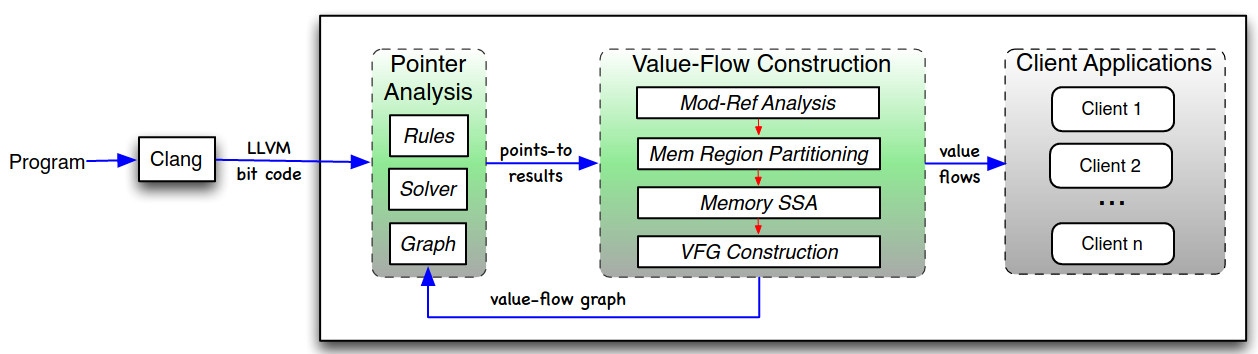
\includegraphics[width=1.\textwidth]{img/svf.png}
    \caption[Overview of the SVF library]{Overview of the SVF library from \cite{sui2016svf}}
    \label{fig:svf}
\end{figure}

Currently, SVF requires version 14 of the LLVM project and makes extensive use of internal data structures.
At the core of the SVF analysis tools is the LLVM-IR which is used to derive information from the source code of a program. Internally this intermediate representation is augmented into the SVF-IR, a graph data structure that models the program assignment graph, short PAG. The PAG is a mostly immutable graph that contains all program instructions and incorporates a model for the memory SSA. All further analyses use the PAG as a root of information from which the analysis results are derived.
See \autoref{fig:pag} for the resulting PAG of the example program in \autoref{tab:applyander}.

\begin{figure}
    \centering
    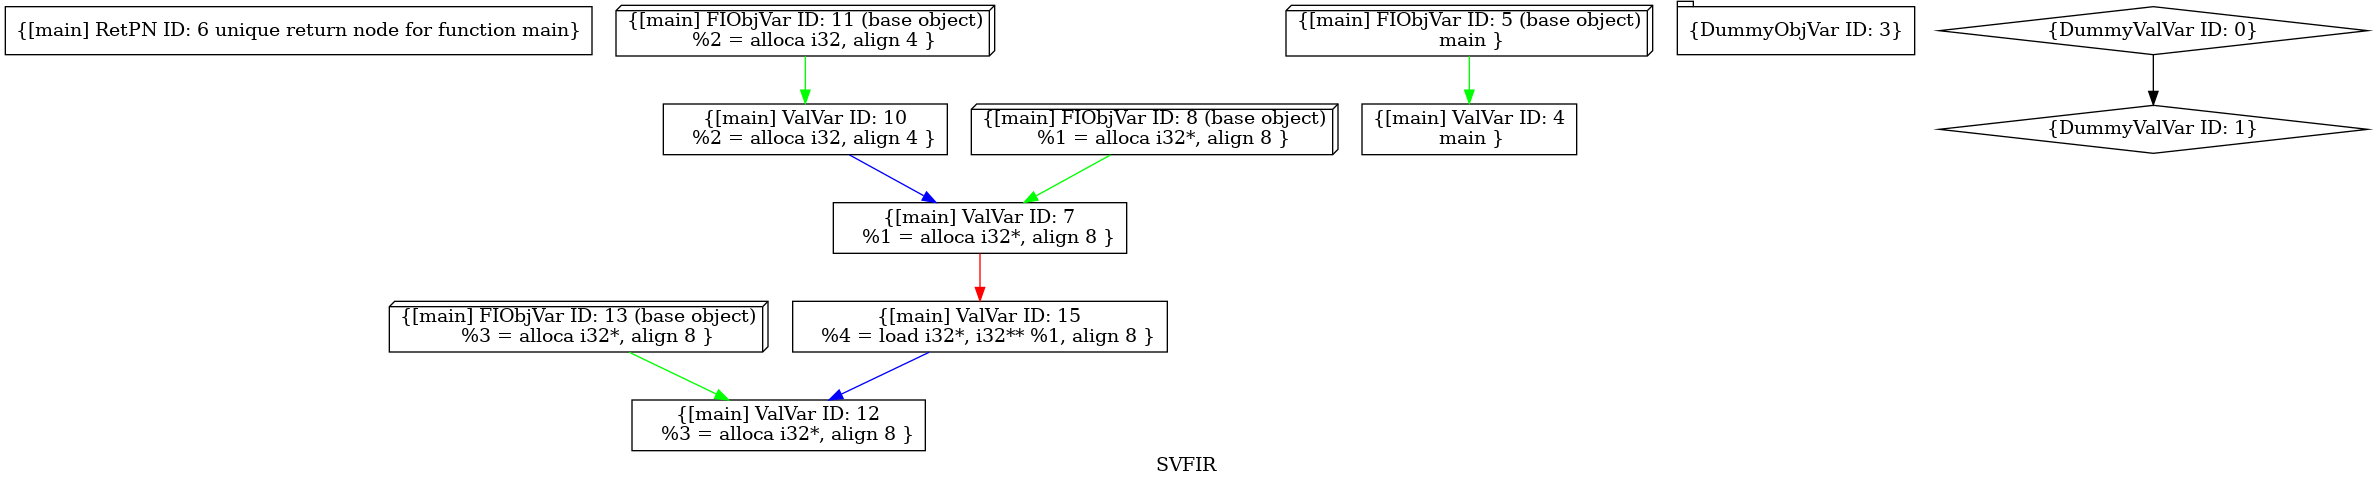
\includegraphics[width=1.\textwidth]{img/pag.png}
    \caption[An example PAG as produced by SVF]{The PAG for the Example from \autoref{tab:applyander} computed by SVF.
        Green edges representing an alloca instruction, blue edges stores and red edges loads.}
    \label{fig:pag}
\end{figure}

The typical analysis run with SVF starts off with a pointer analysis that first derives a constraint graph from the PAG, similar to the procedure described in \autoref{sec:ander}.
The constraint graph is then fed into a pointer analysis algorithm such as the state-of-the-art interprocedural Andersen style Wave Propagation algorithm.
The result is a points-to set for each top-level variable and address-taken variable, as well as a call-graph, that represents an over-approximation for each direct and indirect function call.
Given the points-to information SVF performs an initial mod-ref analysis run to find interprocedural side effects of variables. Given mod-ref and pointer information, defs and uses are then annotated in each procedure with alias sets of abstract memory objects that might be accessed indirectly by loads and stores.
SVF also allows users to specify a memory partitioning strategy whereby the heap can be partitioned with varying granularity to allow for precision and scalability trade-offs.
The properties that are of interest here are specifically the def-use chains of address-taken variables of pointers, which are difficult to compute compared to the def-use chains of top-level variables which are already available if the program in SSA form \cite{sui2016svf}.
The difficulty arises from the seeming ambiguity of indirect accesses to address-taken variables through loads and stores in the program.
After connecting defs and uses of variables, the result is a value-flow graph, or sparse value-flow graph depending on the specified analysis details, that can then be used for more concrete analyses, e.g. use-after-free memory leak detection \cite{sui2014detecting} or fed back into a more precise pointer analysis algorithm to increase precision with the gained value-flow information.

This thesis focuses on pointer analysis, thus, the details of pointer analyses inside SVF are especially relevant. SVF provides a wide set of pointer analyses to choose from, see \autoref{fig:pta-svf} taken from SVF's technical documentation\footnote{\url{https://github.com/svf-tools/SVF/wiki/Technical-documentation}}.
\begin{figure}
    \centering
    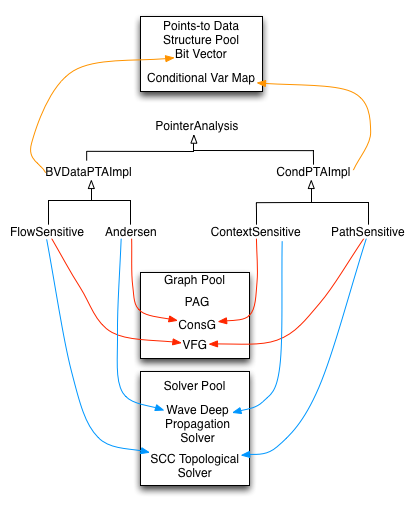
\includegraphics[width=.6\textwidth]{img/pta-svf.png}
    \caption{The class hierarchy of pointer analysis implementations in SVF.}
    \label{fig:pta-svf}
\end{figure}
The components of each implementation can be split into three groups, the Graph, which is a data structure derived from the PAG, that describes where the pointer analysis should be performed.
A set of Rules, which dictate how points-to information should be derived from each statement in the Graph. And a Solver which dictates the order in which the Rules are to be applied on the Graph, according to \cite{sui2016svf}.
A user can then choose which components to reuse and which to replace or augment with custom algorithms or data structures.
This modular approach makes it convenient to experiment with different in-memory representations of points-to data, as well as testing different methods for solving the constraint graph.
\subsection{Graspan}\label{sec:graspan}
Graspan is a disk-based parallel graph system designed for computing transitive closures on very large graphs defined by context-free grammars. It was first introduced by \cite{wang2017graspan} with a CPU backend and later in \cite{zuo2021systemizing} with a GPU based backend.
Disk-based means, that a given constraint-graph is divided into smaller subgraphs, called partitions, that are stored on non-volatile memory and loaded into memory in pairs to calculate the transitive closures in steps that lead to the desired pointer information - or any other static analysis solution that can be defined by a context-free grammar, see \autoref{sec:ander-cfl}.
This approach is similar to many of the design decisions taken by common "BigData" solutions, such as Apache Kafka and Spark, where disk-based solutions are common.

Graspan is meant to be run on a single machine, hence the emphasis on saving memory by offloading to the disk. Another implementation that improves upon the ideas from the Graspan paper is \cite{gu2020towards} where the computation is distributed across multiple nodes, making use of other "BigData" concepts.

Overall Graspan was able to perform a pointer analysis for the Linux kernel in 10.9 minutes with the GPU version \cite{zuo2021systemizing}, while other tools fail to perform on graphs as large as the Linux kernel's constraint graph, which contained 250 million edges after preprocessing and inlining in Graspan. It should be noted that this result was achieved with a flow- and field-insensitive context-free grammar.

In terms of data structures, Graspan has specific requirements. The graph data is large, sparse and dynamic, consequently Graspan uses different in-memory representations for the graph in the CPU and GPU version. The CPU version uses two arrays of $(dst,label)$ pairs that represent the old and new outgoing edges for each node while the GPU version uses a sparse bit vector representation that, while containing the same information as the CPU arrays, is optimized for GPU SIMT parallelism. See \autoref{fig:graspan-g} for an illustration of the GPU optimized sparse bit vector data structure from \cite{zuo2021systemizing}. Internally this GPU optimized data structure is inspired by prior work from \cite{mendez2012gpu}.

\begin{figure}
    \centering
    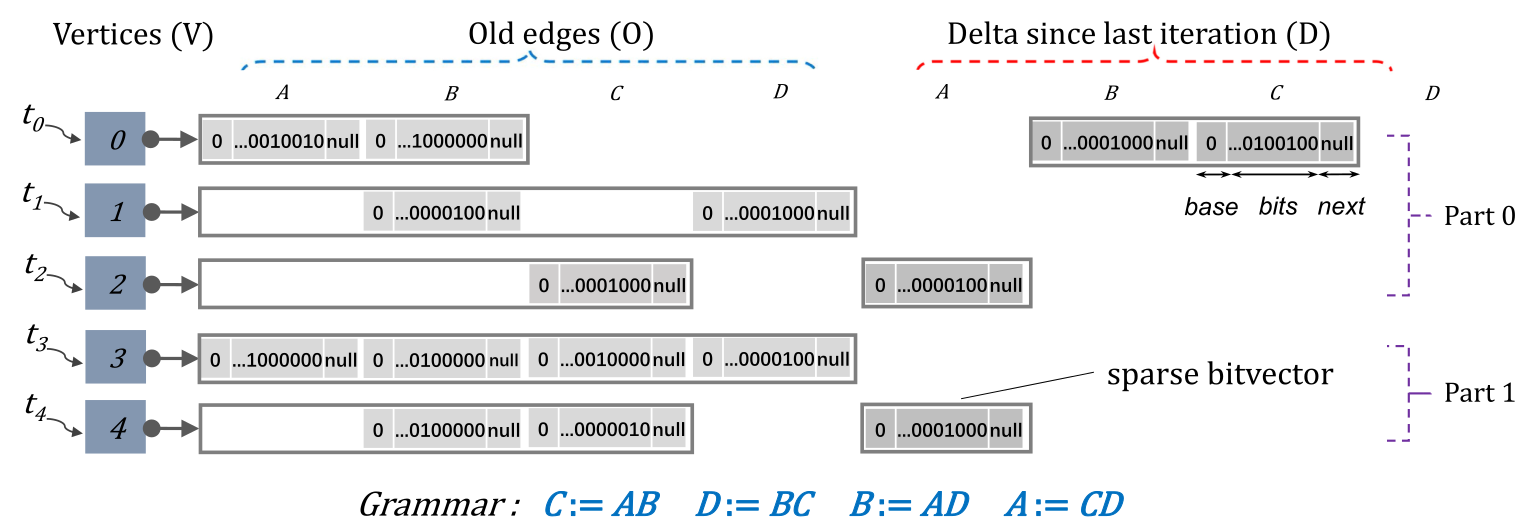
\includegraphics[width=1.\textwidth]{img/graspan-g.png}
    \caption[Graspan GPU Data Structure for the Constraint Graph]{Data structure for the constraint graph in the Graspan GPU version, from \cite{zuo2021systemizing}}
    \label{fig:graspan-g}
\end{figure}

\begin{figure}
    \centering
    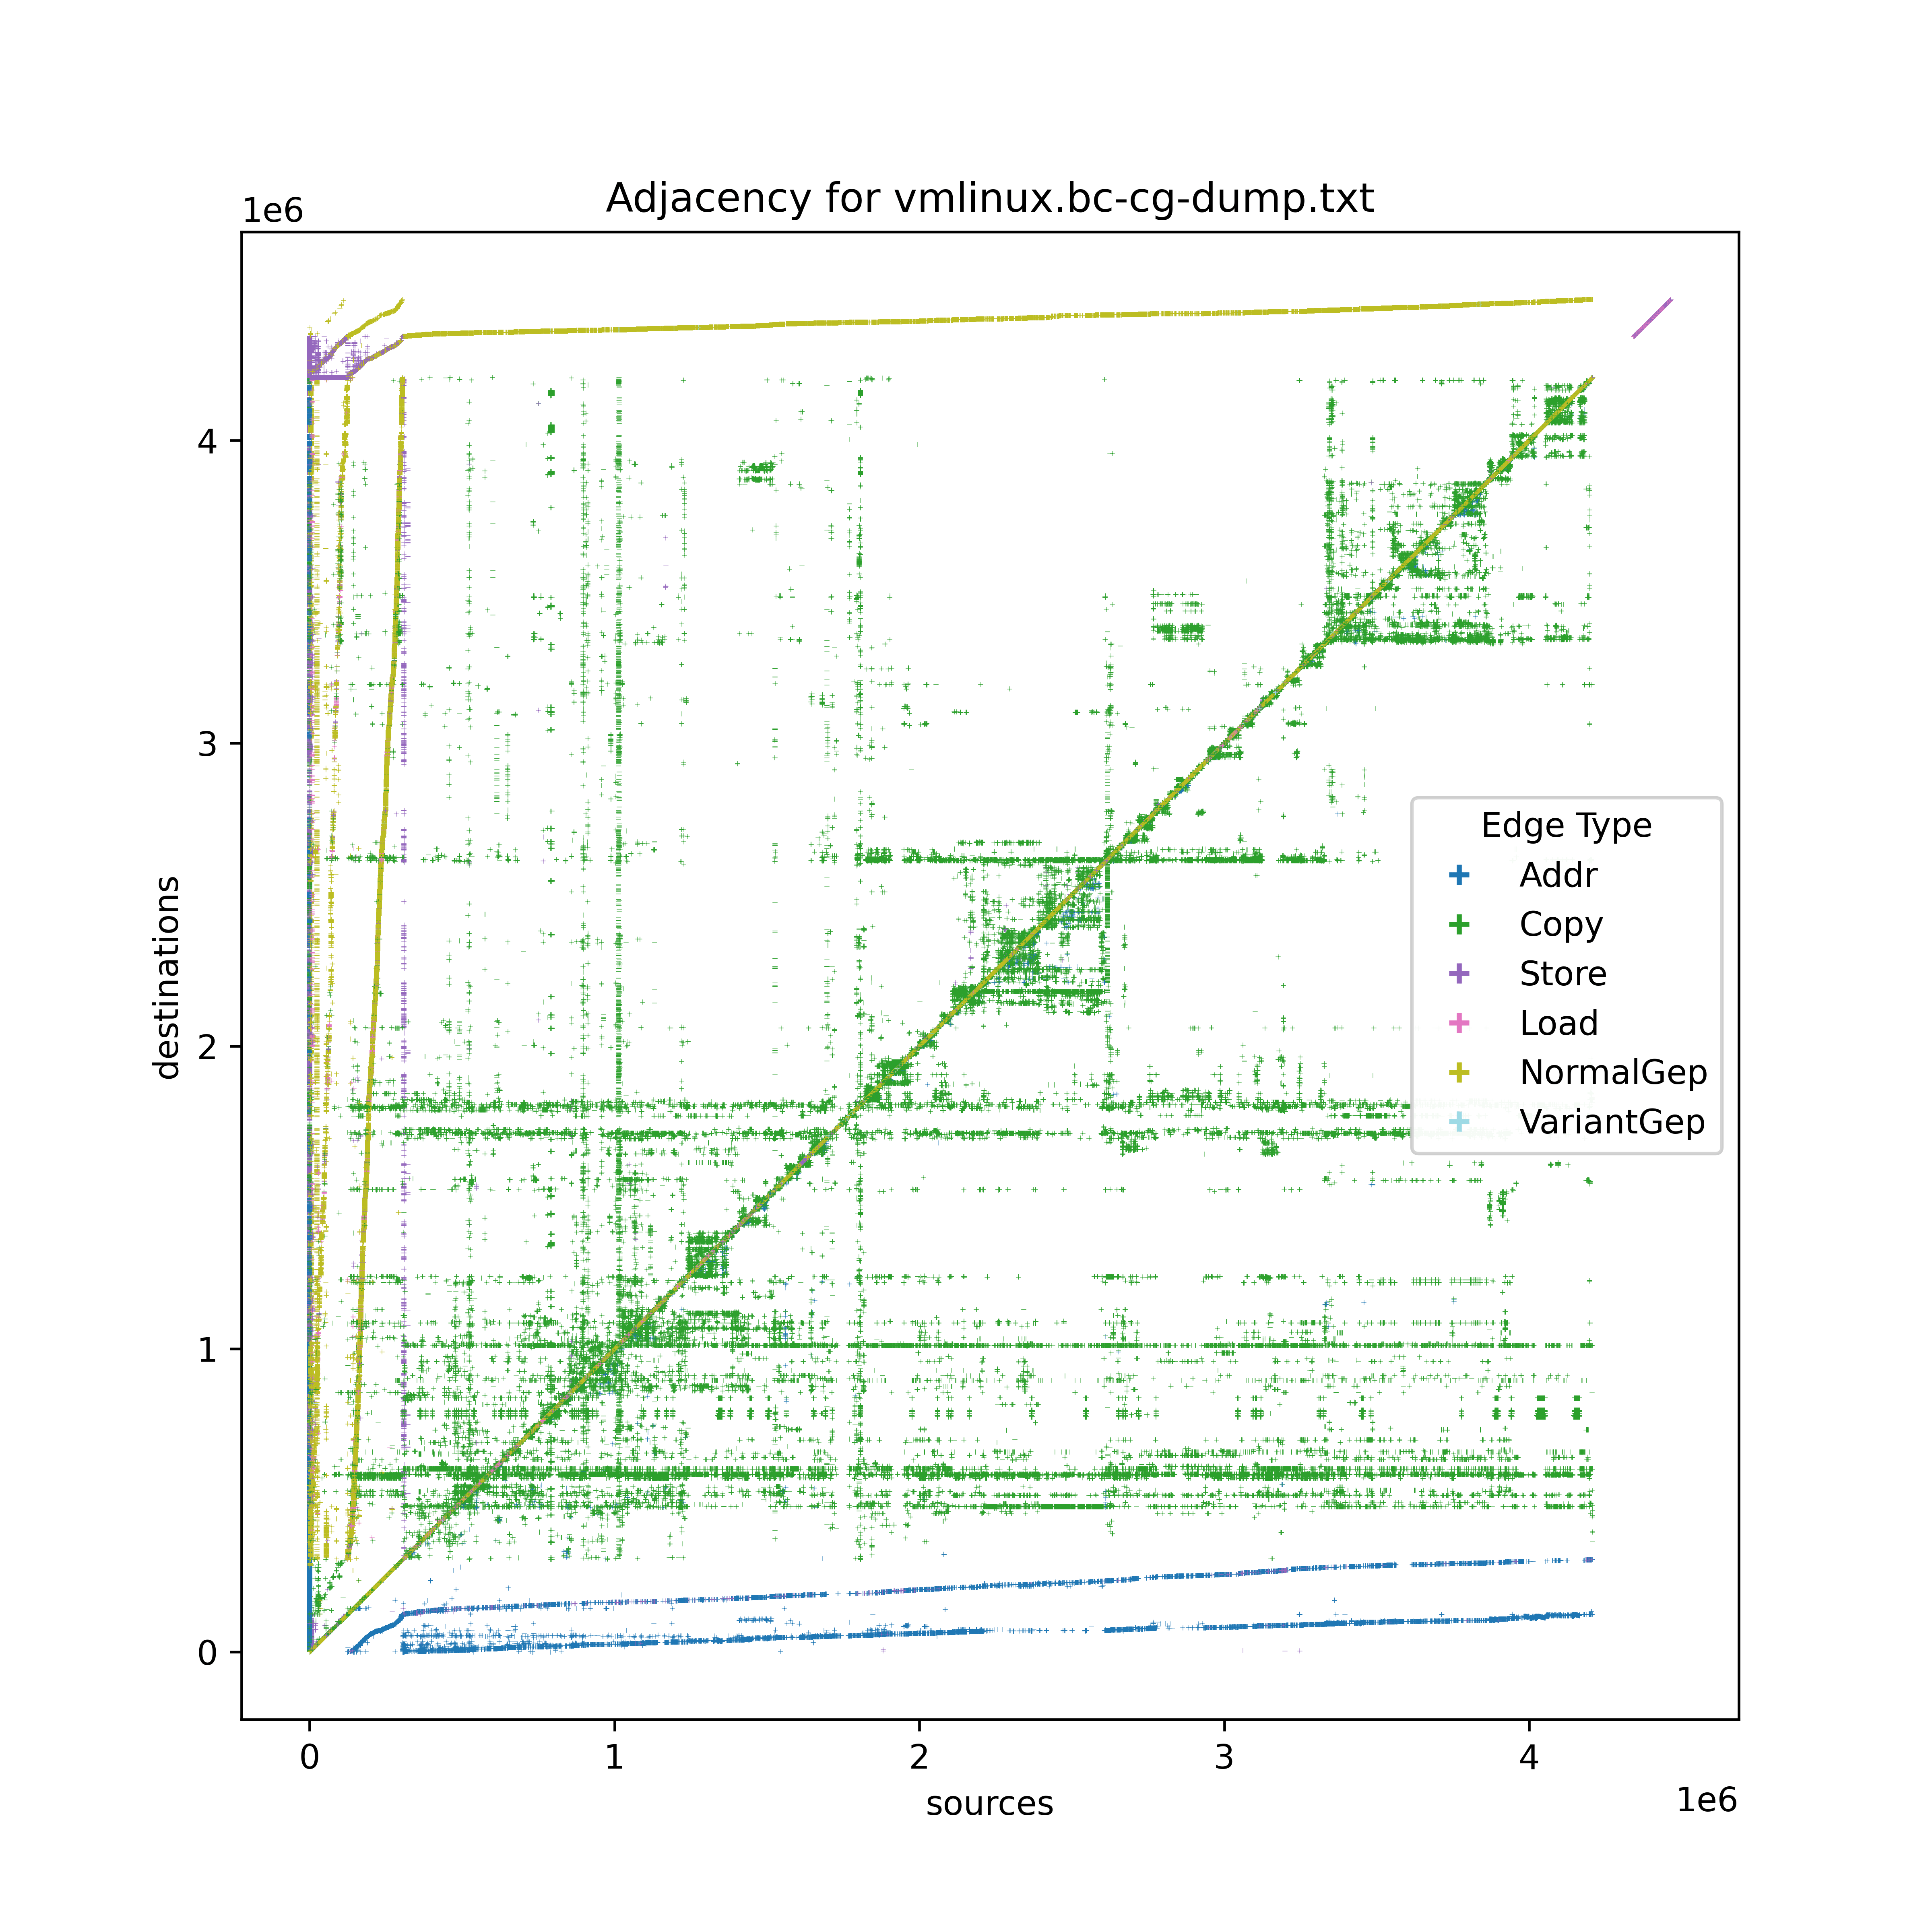
\includegraphics[width=1.\textwidth]{img/linux-consg-min.png}
    \caption{Adjacency Plot for the Constraint Graph of the Linux Kernel}
    \label{fig:linux-consg}
\end{figure}


% \begin{table}
%     \begin{center}
%         \caption{More rows.}
%         \label{tab:table1}
%         \begin{tabular}{l|S|r}
%             \textbf{Value 1} & \textbf{Value 2} & \textbf{Value 3} \\
%             $\alpha$         & $\beta$          & $\gamma$         \\
%             \hline
%             1                & 1110.1           & a                \\
%             2                & 10.1             & b                \\
%             3                & 23.113231        & c                \\
%             4                & 25.113231        & d                \\ % <-- added row here
%         \end{tabular}
%     \end{center}
% \end{table}
